% begin module limits-one-sided-def
\begin{frame}
\begin{definition}[\only<handout:1| -2>{Left}\only<handout:2| 3->{\alert<3>{Right}}-hand\invisible{g} Limit]
We write
\[
\lim_{x\rightarrow a^{\only<handout:1| -2>{-}\only<handout:2| 3->{\alert<3>{+}}}}f(x) = L
\]
and say the \only<handout:1| -2>{left}\only<handout:2| 3->{\alert<3>{right}}-hand limit of $f(x)$ as $x$ approaches $a$ is equal to $L$ if we can make the values of $f(x)$ arbitrarily close to $L$ by taking $x$ to be sufficiently close to $a$ and \only<handout:1| -2>{less}\only<handout:2| 3->{\alert<3>{greater}} than $a$.
\end{definition}
\begin{columns}[c]
\column{.5\textwidth}
\ 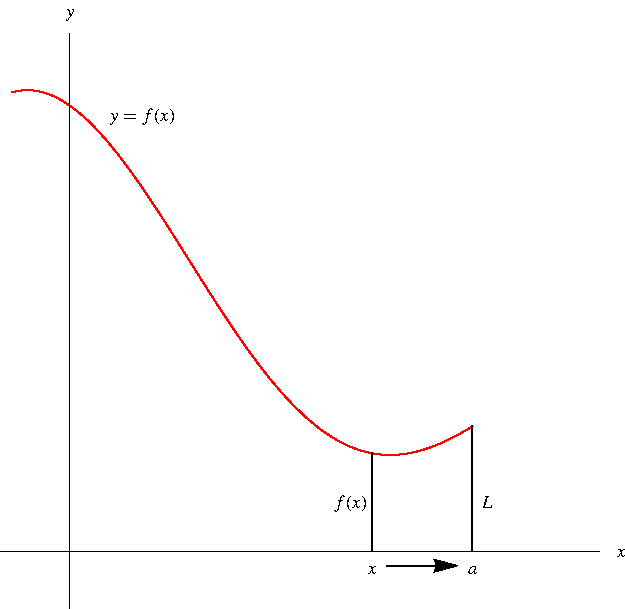
\includegraphics[height=4cm]{limits/pictures/02-02-leftlim.pdf}%
\column{.5\textwidth}
\uncover<handout:2| 3->{%
\ 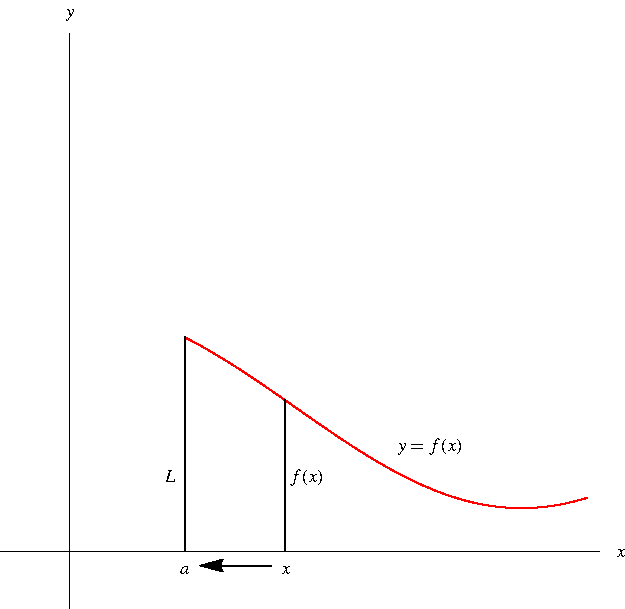
\includegraphics[height=4cm]{limits/pictures/02-02-rightlim.pdf}%
}%
\end{columns}
\uncover<handout:2| 2->{%
We can define a right-hand limit similarly.
}%
\end{frame}
% end module limits-one-sided-def
